Weather conditions have a huge impact on the electricity industry in terms of network infrastructure and electricity consumption. In \cite{19} they describe a multiple regression model that accurately predicts the monthly electricity demand based on weather and sociocultural conditions. The monthly electricity demand from this model shows a clear cyclic pattern which reflects the temperature changes during the year \cite{19}. Besides weather conditions, social and economic factors also affect the monthly demand, e.g. the demand was decreased in Denmark during the financial crisis in 2009 \cite{20}. 

\subsubsection{Parametric multiple regression}
Parametric multiple regression is preferred in \cite{19} as opposed to an Artificial Neural Network used in this thesis. From a statistical error indices point of view the Artificial Neural Network (ANN) is a valid choice for prediction (see figure ~\ref{fig:anncomparison}) in relation to the error. The argument for multiple regression is the simplicity in adjusting input values for each analysis of electricity demand in the prediction model and in the end they show similar results to ANN. 
\begin{figure}[h!]
\centering
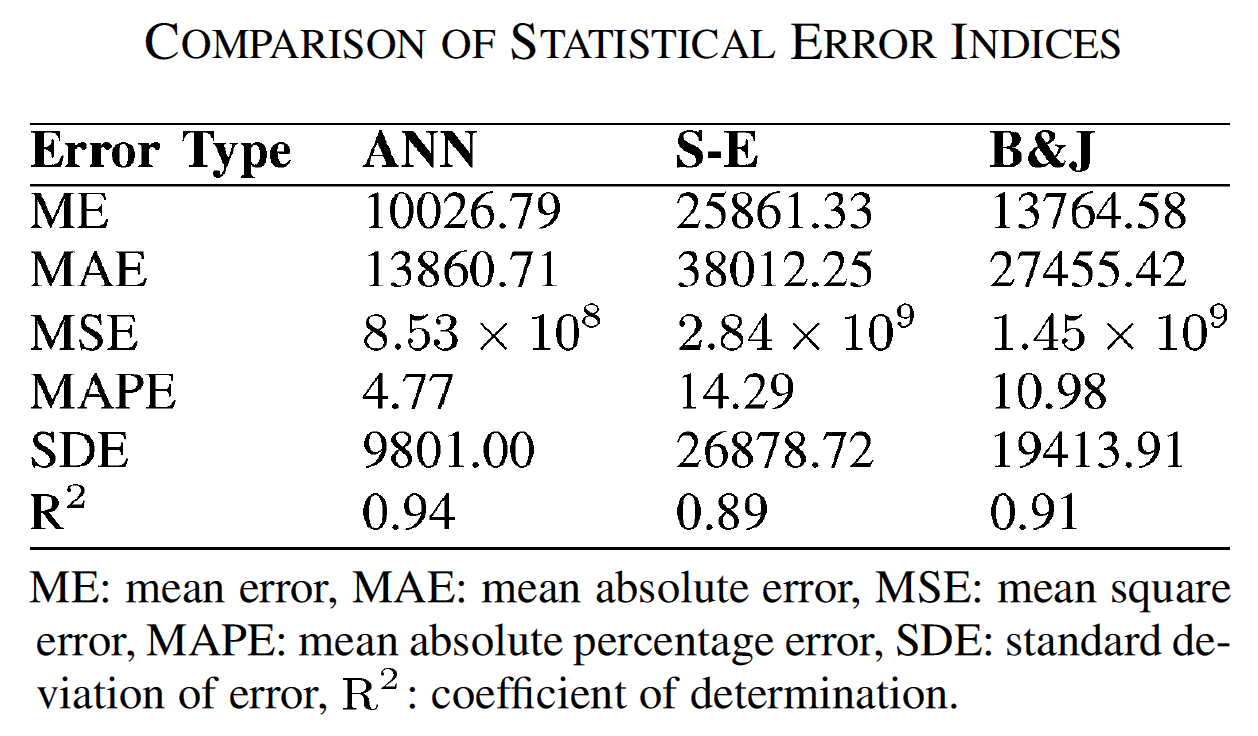
\includegraphics[width=0.8\linewidth,natwidth=898,natheight=587]{billeder/StatisticalErrorOfNeuralNetworksAndRegression.png}
\caption{Shows ANN compared to B\&J and SE \cite{19} }
\label{fig:anncomparison}
\end{figure}
To make a demand prediction based on weather conditions a relationship between the two needs to be established. To get an understanding of this relationship, a plot of the average monthly demand as a function of Central England Temperature (CET) can be made \cite{19}. The plot (see figure ~\ref{fig:CET}) shows an inverse relationship where it can be seen that a lower temperature in general results in an increased load consumption. Winter gives rise to lighting and heating load which is consistent with lower temperatures, and conversely in the summer with temperatures above 18 degrees the consumption tends to increase again due to the need for cooling and air-condition \cite{19}.
\begin{figure}[h!]
\centering
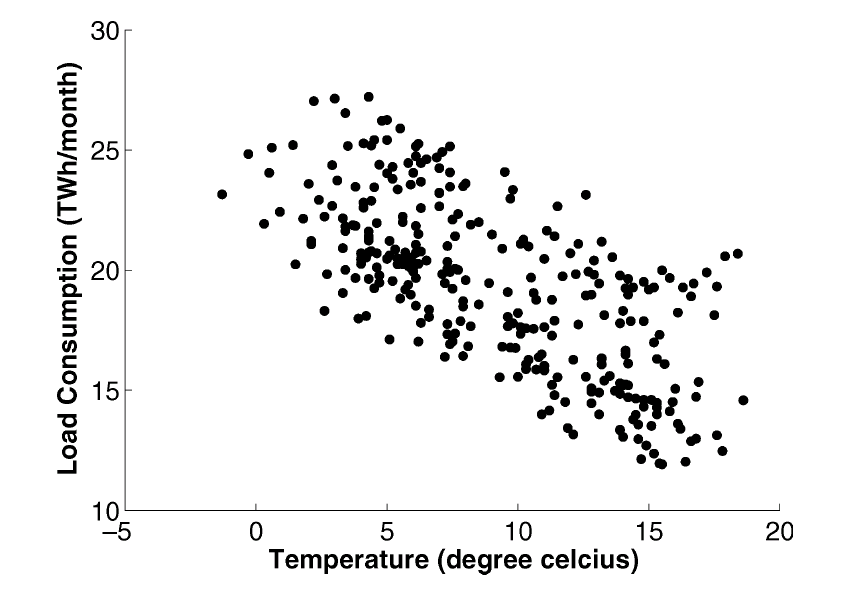
\includegraphics[width=0.8\linewidth,natwidth=898,natheight=587]{billeder/MeanMonthlyDemandEngland.png}
\caption{Function of monthly CET as a function from 1970 to 1995 \cite{19}}
\label{fig:CET}
\end{figure}

\subsubsection{Heating and Cooling Degree Days}
The nonlinear relationship between temperature and load consumption is turned into a concept called degree days. They introduce two categories of days; 1) Heating Degree Days (HDD) that is used to quantify when heating is required; 2) Cooling Degree Days (CDD) which is then used to quantify the need for cooling. The days are calculated from the CET data and give a more indicative picture than the temperature-load relationship \cite{19}. A simple explanation of the calculation follows.
\begin{center}
$CDD=\sum\limits_{d=1}^{N_{d}}(\gamma_{d})(T_{dm}-T_{base_{C}})$
\end{center} 
 
where $T_{base_{c}} = 20^{\circ}$ is the base temp and $T_{dm}$ is the mean daily temperature. $\gamma_{d} = 0$ if $T_{dm}-T_{base_{c}} < 0$ and $\gamma_{d} = 1$ if $T_{dm}-T_{base_{c}} > 0$. In other words if the temperature if above $20^{\circ}$ the day can be characterized as CDD and there is a need for cooling.
\begin{center}
$HDD=\sum\limits_{d=1}^{N_{d}}(1-\gamma_{d})(T_{base_{H}}-T_{dm})$
\end{center} 

where $T_{base_{h}} = 15.5^{\circ}$ is the base temp and again $T_{dm}$ is the mean daily temperature. $\gamma_{d} = 1$ if $T_{base_{h}}-T_{dm} < 0$ and $\gamma_{d} = 0$ if $T_{base_{h}}-T_{dm} > 0$. This means that on a day with temperatures below 15.5 degrees there is a need for heating. In both cases where $\gamma_{d} != 0$ a big difference has a greater impact on the demand.

Temperature is the most influential factor but other weather conditions can also be used when calculating the electricity demand, e.g. wind speed and rainfall can impact heating and lighting demand whereas direct sunshine can decrease the need for heating \cite{19}. The model can be expressed by the relation between all factors by adding them together, e.g. the HDD value automatically increase the total electricity demand if it is not zero and this apply to all other factors in the model seen below.

\begin{center} \^E$_{A}=\alpha_{0}+\alpha_{1}CDD+\alpha_{2}HDD+\alpha_{3}ELD
+\alpha_{4}V_{w}+\alpha_{5}M_{s}+\alpha_{6}M_{r}$ 
\end{center} 
 
Where $\alpha_{n}$ are constants, ELD is humidity, $V_{w}$ is wind speed, $M_{s}$ sunshine and $M_{r}$ rainfall.
The calculation model can also include socio-economic factors. Specifically the population growth has a natural impact on the electricity demand over time. The more people the higher the demand gets. This would give rise to an additional factor in the model considering the growth. The prediction model from \cite{19} comes within 3 percentage of the actual demand when it is run on data from 1996-2003 which is pretty close (~\ref{fig:predicteddemand}).
\newline
\begin{figure}[h!]
\centering
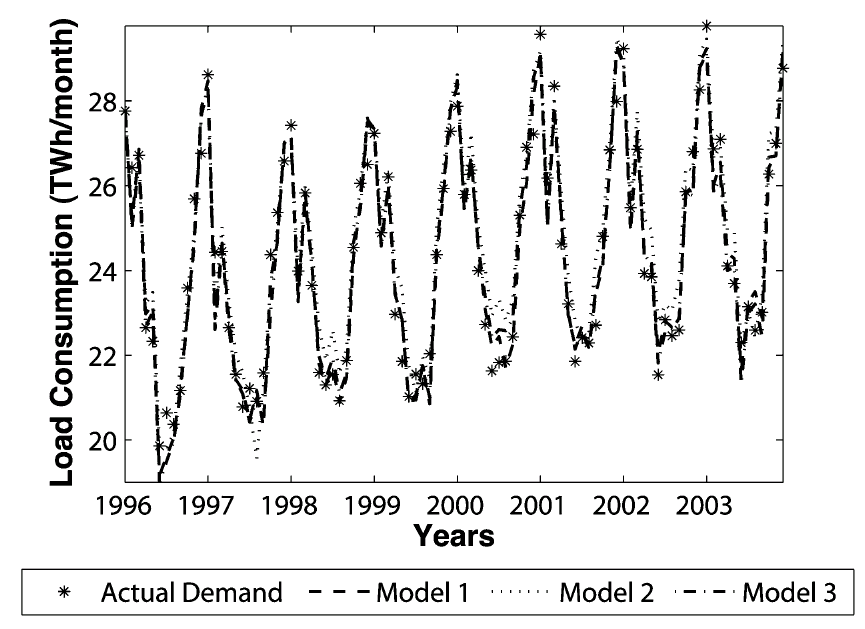
\includegraphics[width=0.8\linewidth,natwidth=898,natheight=587]{billeder/PredictionOfDemand.png}
\caption{The actual values and the predicted demand in a comparison \cite{19}}
\label{fig:predicteddemand}
\end{figure}

\subsubsection{Summary}
The electricity demand has great influence on the energy price. It is important to identify the influences of the demand because those inevitably also will have an affect on the electricity prices. 

The concept of Cooling Degree Days (CDD) and Heating Degree Days (HDD) has been described. It could be interesting to see the result on accuracy when using these simple calculations on the temperature input because it simply ignores the temperature when heating or cooling is not needed. It also needs to be discussed if the concept of degree days makes sense in countries without heating or cooling tradition.
Furthermore the demand function (\^E$_{A}$) is presented. This function gives an exact picture of the factors that directly influence the demand and the possible mappings to our ANN as the demand part --- every parameter is an input.